%%% template.tex
%%%
%%% This LaTeX source document can be used as the basis for your technical
%%% paper or abstract. Intentionally stripped of annotation, the parameters
%%% and commands should be adjusted for your particular paper - title, 
%%% author, article DOI, etc.
%%% The accompanying ``template.annotated.tex'' provides copious annotation
%%% for the commands and parameters found in the source document. (The code
%%% is identical in ``template.tex'' and ``template.annotated.tex.'')

\documentclass[annual]{acmsiggraph}

\TOGonlineid{45678}
\TOGvolume{0}
\TOGnumber{0}
\TOGarticleDOI{1111111.2222222}
\TOGprojectURL{}
\TOGvideoURL{}
\TOGdataURL{}
\TOGcodeURL{}

\title{Auto Feature Selection for Object Detection, Can or Can't?}

\author{Bao Nguyen Thien\thanks{e-mail:ntbaovn@gmail.com}\\ 
        Yoshiaki Shirai\thanks{e-mail:shirai@ci.ritsumei.ac.jp} \\
        Graduate School of Information Science and Engineering\\
        Ritsumeikan University, Japan
}
%%\pdfauthor{Robert A. Smith}

\keywords{feature seclection, object detection, image processing, computer vision
%%radiosity, global illumination, constant time
}

\begin{document}

%% \teaser{
%%   \includegraphics[height=1.5in]{images/sampleteaser}
%%   \caption{Spring Training 2009, Peoria, AZ.}
%% }

\maketitle

\begin{abstract}
This research focuses on developing a system that can retrieval objects from large image database by exploring the
types of image features necessary for recognition of common objects in scene. Then we make global representation for these
features that can be used in learning. After that, we figure out a novel method for generic object detecting in still images with automatically choosing feature. Our method is simple, computationally efficient and bases on features that is easily seen by naked-eye and very close with natural detecting by human. The main advantage of this method is that it can automatically choose features which are best for detecting one type of object. We present experimental results for detecting many visual categories including side view car, front view car, bike, motorbike, train, aero plane, horse, and sheep. Results clearly demonstrate that the proposed method is robust and produces good detection accuracy rate.
\end{abstract}



\begin{CRcatlist}
   \CRcat{I.4.8}{Image processing and computer vision}{Scene Analysis}{Object recognition}
   \CRcat{I.5.2}{Pattern Recognition}{Design Methodology}{Feature evaluation and selection};
\end{CRcatlist}

\keywordlist

\TOGlinkslist

\copyrightspace

\section{Introduction}
\label{sec:introduction}
The amount of visual information available in digital collections
increases every day. Pictures, medical images, graphs and photos
among others are collected for books, papers, diagnosis, reports,
news, albums, etc. Due to this, Content-Based Image Retrieval
(CBIR) has recently become an active research discipline. Despite
the advances in content-based image retrieval, different problems
remain unsolved. The main problem is the semantic interpretation of
the image content~\cite{smeulders2000content}. Most of CBIR systems try to work on
semantic of image. But the semantic is not easy to get. There are
many solutions for understanding the content of image. The easiest
way is to describe image with text annotation. There are different
situations in which images are surrounded by text descriptions that
may provide contextual hints or semantic information about their
contents. In this approach, image semantics are learned from an
external source such as user feedbacks and textual annotations, and
of course both are provided by human beings. 
However, learning from external sources is limitted because we have no
annotation is correct or not. Moreover, there are different scenarios
in which descriptive annotations are not available for all images in
the collection or the user is not able to provide an accurate textual
query. Furthermore, several works have shown that, even in the
presence of text descriptions, visual features are useful
information source to identify relevant images in a large scale CBIR
system, showing important improvements in performance~\cite{jing2007canoical,grubinger2008advances}.
In this research, to understand the semantic of image, instead of
annotation, we base on objects in the image. The more objects a
system can detect, the more precise that system is. Object detection
and recognition is still a difficult problem for computer vision. Most
methods base on features of an image including both local and
global one for detecting object. The goal of this research is to
develop a necessary methodology for recognition of general object
in still images by automatically choosing features. We base on
features that are easily with natural recognizing by human. Most
state-of-art methods focus on how to recognize object after fixing
some features. In contrast, in this research, we let system choose
features from a list of features, and the system determines by itself
which features are good for detecting a given object.

The rest of this paper is organized as follows. Section~\ref{sec:related_works} discusses
previous work related to the approach taken here. Section 3
describes the set of attributes we use, and how we create attribute
classifiers. In section 4 we propose an algorithm for automatically
choosing best features. In our experiments (section 5) we first
evaluate the performance of both the individual attribute classifiers
and combination attribute classifiers. We also compare the attribute features 
with other methods. Result of automatically choosing features is also presented in this part.
The last section discusses experiment results and suggests some future directions.


\section{Related Works}
\label{sec:related_works}
The most popular approach for object classification is to extract
local regions from images, assign them to clusters, and use the count
distribution across clusters as an input to a general classifier[4].
Some other approaches try to locate the object within the image, and
to take into account the spatial relationship of the image regions
which trigger potential matches~\cite{ferrari2008learning}. These methods, however, tend to
have high computational complexity. The 'bag of words' approach,
instead, uses the histogram of counts across the whole image to
predict whether or not the image contains the class of interest. While
the image background may create confusion in recognizing object
classes, the background can also provide useful cues to aid
recognition [9]. Simple bag-of-words methods have shown
impressive performances for object classification when used with
large number of region descriptors and optimized parameters~\cite{marcin2007learning}.

The local features used in bag-of-words methods typically lack
any clear semantic meanings. The individual features do not usually
have strong discriminative power, and the methods perform best
when provided with very high-dimensional image descriptors.
These descriptors allow the discovery of significant differences
between different class feature distribution. Learning features
with more specific meanings might help improve classification
performance. Some previous work has looked at explicitly learning
semantically meaningful features. For example, Van de Weijer et al.~\cite{van2009learning} learnt to map from image color to the color names people use to describe objects. 
Ferrari and Zisserman~\cite{ferrari2007learning} also learn simple texture attributes such as 'stripes' or 'dots'.
Recent work has embraced more complex attributes. Vogel and Schiele~\cite{vogel2004natural} used attributes
describing scene, material, and shape to retrieve images of coasts,
rivers/lakes, forests, plains, mountains, and sky/clouds.
Farhadi et al.~\cite{farhadi2009describing} used a set of semantic attributes such as 'hairy' and 'fourlegged' to identify familiar objects, and to describes unfamiliar objects when an image and a bounding box annotation are provided.
Lampert et al.~\cite{larmpert2009learning} showed that high-level descriptions in terms of
semantic attributes can be used to recognize object classes without
any example images, once semantic attribute classifiers are trained from other classes.

We also use diverse semantic attributes with explicit meanings to
describe the visual content of images. Notable differences include
that most of these approaches based on both local and global features
difficult to see with human eyes. In our method, we base on features
that are easily seen and very close with human. Moreover, these
attributes provide contextual information which is important for 
object classification. Beside, we do not use any manual semantic
attribute labels for images, instead collecting a separate set of
representative images. Our system automatically decides which
feature is good to recognize for a specific object. The classifiers
learnt in this way are more general than all other approaches which
fix features before detecting.









\section{Object Dectection Based on Combination of Multiple Features}
\label{sec:objectdetection}
In the first stage, we try to detect object by combination many
features including both global and local features. Up to present, we
have tested with seven features, such as: edge, corner, HoG, line,
circle, SURF, and color. This section describes how to extract and use
these features for recognize object.
\subsection{Edge, Corner and HoG Feature}
It is easy to see that the most important features for recognition
object are the overall shape of that object and all boundaries which
separate main parts of object. Shape or boundary is basically
composed by edges. These edges are arranged in a specific order and
meet each other at some points called corners. Beside, edge
orientation also plays a prominent role for figuring object. With the
same number of edges, but in different order and different orientation,
it makes viewer imagine different objects. The description of how
these principal components make object imaginable is in Fig.~\ref{fig:3components}.
\begin{figure}[ht]
  \centering
  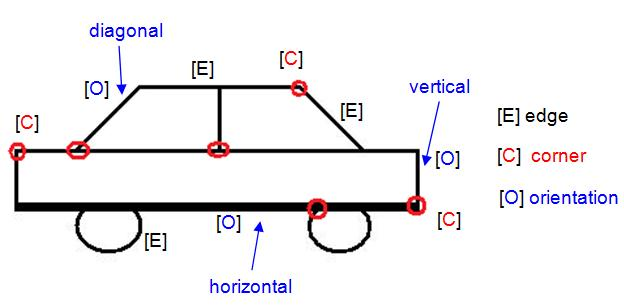
\includegraphics[width=2.20in]{images/edge_cornre_HoG.jpg}
  \caption{Three main components make object be figured.}
  \label{fig:3components}
\end{figure}

Based on this, we propose an overall approach for object detecting
which focuses on edge, corner and edge orientation (HoG). More
detail is presented in the next diagram in Fig~\ref{fig:framework}. But there is still an
issue in this model. That is how do we know that edge/corner is at
right position or not? In order to answer this question, we must point
out the place where edge/corner must belong to before detecting
object. Actually, there are many way to specify location of
edge/corner, such as using prior knowledge, or machine learning, etc.
\begin{figure}[ht]
  \centering
  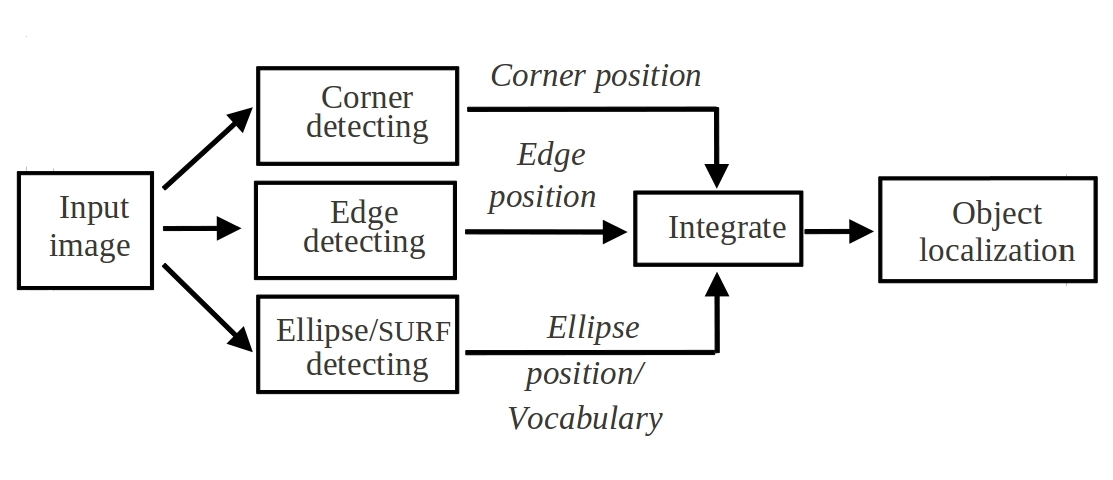
\includegraphics[width=3.15in]{images/framework1.jpg}
  \caption{Object detection based on multiple features.}
  \label{fig:framework}
\end{figure}
In our implement, we choose machine learning approach because
it is more general for a lot of objects and one most
important reason is that it requires no user's prior knowledge about object that they want to detect.

\textit{Edge and corner detection }
Up to present, there are a lot of implementations of edge/corner
detection and get the result with a high accuracy rate. Many of them
have been reported in public. Zuniga and Haralick fit a continuous
surface over a small neighborhood of each point and consider the
rate of change in gradient direction. Moravec defined 'points of interest' as points where there is a 
large intensity variation in every direction. Harris and Stephens used image derivatives to estimate the
autocorrelation of the image. Rangarajan, Shah and Brackle found an
optimal function representing the corner detector which when
convolved with the gray level function yields a maximum at the
corner point. Rafajlowicz, E. uses the idea of vertically weighted
regression and in its simplest form it leads to interpreting SUSAN in
terms of a box sliding on the surface of an image. This modification
of the SUSAN algorithm is still simple, robust against errors and
provides thinner edges, without further efforts on additional thinning.
Canny introduces the notion of non-maximum suppression, which
means that given the pre-smoothing filters, edge points are defined
as points where the gradient magnitude assumes a local maximum in
the gradient direction. Sonya Coleman et al~\cite{coleman2007integrated}
proposed a new method for enabling edge and corner detection to be
integrated with a significantly reduced computation time.
In our performance, we have tried with many methods for
edge/corner detecting, and Canny detector gave the
best result for edge detection, while Harris detector worked well with
corner detection.

\textit{Edge orientation detection }
Specifying orientation of each edge is not an easy task. Because,
with all edge detection method above, we only get the total edge
image not each separate edge in image. So, it is almost impossible to
know the orientation of each edge due to we don t specify each edge
individually. Instead of that, we can calculate the domain orientation
of all edge in a specific sub-image. From this, we can define
relatively the edge orientation. The domain orientation of a region
can be calculated with HOG descriptor method (Histogram of
Oriented Gradient). HOG descriptor is a local statistic of the
orientations of the image gradients around a keypoint. HOG
descriptor was initially proposed by Lowe in his Scale Invariant
Feature Transform (SIFT)~\cite{lowe2004distintive}. Several HOG-based algorithms have
been recently presented~\cite{bay2008surf} and combined with technologies such as
boosted classifiers~\cite{dalal2005histograms}, in which Navneet Dalal and Bill Triggs (INRIA) have
used this method for human detection with a high accuracy rate.
David Monzo et al~\cite{monzo2008hog} compared HOG-EBGM vs. Gabor-EBGM
and showed the result that HOG had a better performance.

\textit{Making edge map and corner map }
\textit{Edge map/corner map} is used to know if edge/corner is at right
position or not. To make edge map and corner map, we use the same
method as Zhenfeng Zhu et al~\cite{zhu2004car}. For all images in the positive
training-image set ($T_{pos}$) (the rest of training-image set is negative,
$T_{neg}$), after detecting edge/corner we accumulate them in one temp
image $T_{e}$ or $T_{c}$. Then edge map and corner map will be made from
these temp images respectively. However,~\cite{zhu2004car} makes edge map and
corner map be binary images. Our performance shows that with gray
scale image, the result will be better. With a binary map, the location
of edge or corner must be fixed at that position. But, due to variant
of scale or view point, the location of edge or corner cannot be fixed
at one specific point, other while it can be swung in a small region.
Intuitively, gray scale map works better in this case.
\begin{figure}[ht]
  \centering
  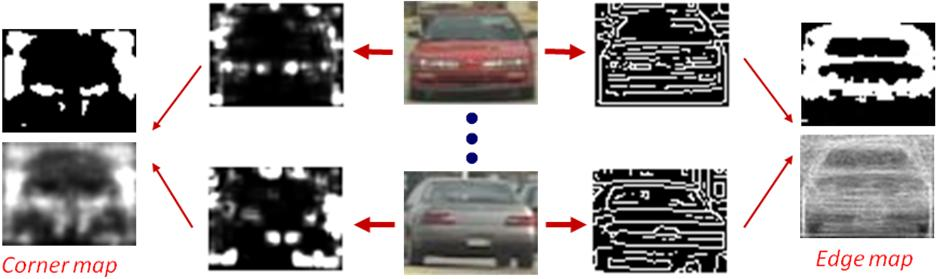
\includegraphics[width=3.25in]{images/edgemap_cornermap.jpg}
  \caption{Making Edge map and Corner map from training set.}
  \label{fig:making_edge_corner_map}
\end{figure}
The edge map $M_{E}(x,y)$ and corner map $M_{C}(x,y)$ are constructed from
$T_{e}$ and $T_{c}$ as following
\begin{equation}
M_E(x,y) = \frac{T_{e}(x,y)}{\theta_1 \times N} \mbox{~~~~and~~~~}
M_C(x,y) = \frac{T_{c}(x,y)}{\theta_2 \times N}
   \label{eq:edge_corner_map}
\end{equation}
where $N$ is the number of images in the training set; $\theta_1, \theta_2$ are
specific thresholds. %hreshold $\theta_1$ equals to 25 and value 35 is for $\theta_2$. 
\subsection{SURF Feature}
In order to increase the accuracy rate, after a candidate satisfies edge
map, corner map and orientation of edge, that candidate is continuously
passed to SURF~\cite{bay2008surf} checking stage. We choose SURF because it
is invariant with scale, illumination, and similar but faster than SIFT.
\begin{figure}[ht]
  \centering
  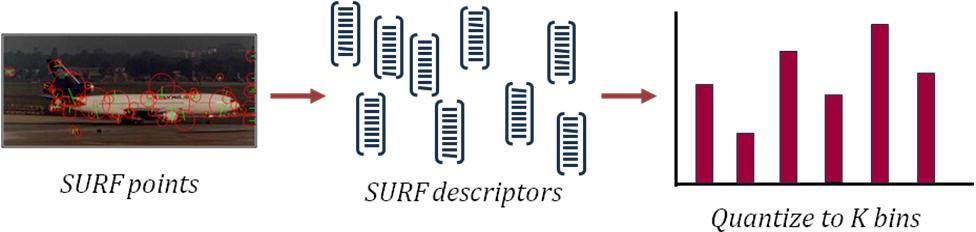
\includegraphics[width=3.25in]{images/surf.jpg}
  \caption{Making vocabulary for matching SURF feature.}
  \label{fig:making_surf}
\end{figure}
Method of matching between two set of SURF descriptors as
Gabriella et al in\cite{lazebnik2006beyond,csurka2004visual} is used. Bag of keypoints or vocabulary
are made by quantizing all descriptors from training image set to K
bins. Once descriptors have been assigned to form feature vectors,
we use Naïve Bayes classifier to determine whether an input image
belongs to one category or not by taking the largest posterior score,
$argmax\{P(C_j|I)\}$
\begin{equation}
   P(C_j|I) \propto P(C_j)P(I|C_j)= P(C_j)\prod_{t=1}^{k} N^{(t,I)} P(v_t|C_j)
   \label{eq:surf}
\end{equation}
where $I$ is new image, $C_j$ is category class (object/non-object), $v_t$
represents for keypoint or cluster center, and $N^{(t,I)}$ is the number of
times that keypoint $v_t$ occurs in image $I$.
\subsection{Color Feature}
With some objects such as horse, sheep,
their color changes not much. Color is then
a good point to distinguish object and non-
object. We mark which color belongs to
object by making color map from training
images after converting to HSV space.
Follow is an example of horse color map
from all HSV images. Inside the yellow
boundary is horse-color region, other
while outside is non-horse color region.
Color matching is calculated by
\begin{figure}[ht]
  \centering
  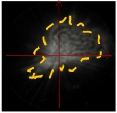
\includegraphics[width=0.90in]{images/colormap.jpg}
  \caption{Horse color map.}
  \label{fig:horse_color}
\end{figure}
\begin{equation}
   M_{color} = \sum_{x,y} CM(x,y) * H(x,y)
   \label{eq:color}
\end{equation}
which $CM$ is color map and $H$ is histogram of image in $HSV$ space.
After extract feature, in order to determine feature is used for
detecting a specific object or not, we should know if that feature
satisfies object. Value of feature $f$ in an image $i$ is written as $val(f,i)$.

\textit{Definition 1:} With a given image $i$, one feature $f$ is called satisfy ,
written as $sat(f,i)$, if the value of feature $f$ in image $i$ falls into the range of all
values of $f$ in the set of positive images - $T_{pos}$
\begin{equation}
   {argmin}(val(f,i_{pos}) \leq val(f,i) \leq {argmax} (val(f,i_{pos})
   \label{eq:sat_f}
\end{equation}
with all images $i_{pos} \in T_{pos}$

\textit{Definition 2:} A given image $i$ is called satisfy a feature set $F$,
written as $sat(F,i)$, if the image $i$ satisfies all features $f$ of $F$
\begin{equation}
   sat(F,i): \forall f \in F, sat(f,i) = True
   \label{eq:sat_F}
\end{equation}
\textit{Definition 3:} With a given image set $I$, and a feature set $F$, a subset of $I$ satisfying $F$ is called $sat(F,I)$ 
\begin{equation}
   sat(F,I) = \{i \in I, sat(F,i)\}
   \label{eq:sat_F_I}
\end{equation}
We only describe Edge, Corner, HoG, SURF and Color feature.
With Circle feature, Line feature we use Hough Transform to extract. In the next section, an algorithm for automatically determining which feature to be good to recognize a given object is presented.







\section{Automatic Feature Selection}
\label{sec:feature_selection}
Instead of choosing features manually before detecting object, we propose an algorithm for automatic feature selection to determine which features be useful for a specific object. Automatically choosing
feature is the most advatage of our system. In most of the other state-
of-art recognizing object systems, the designer must define features
which are used in their system. This is a limitation
because the system has to work with one or some specific features,
while other strong features for object cannot be used. Due to this,
automatically choosing feature is a novel contribution to the pattern recognition literature. 

Init:\mbox{~~~~~~~}$F_c = \o$, set of chosen features\\
\mbox{~~~~~~~~}\mbox{~~~~~}$F = \{f_i\}$, set of all features

Step 1:\mbox{~~}$\forall f_i \in F$\\
\mbox{~~~~~~~~~~~~~}$g(f_i,F_c) = \omega_p * pos(f_i,F_c) + \omega_n * neg(f_i,F_c)$

\mbox{~~~~~~~~~~~~} where: $ pos(f_i,F_c) = |sat(F_c \cup \{f_i\}|T_{pos})| * 1/|T_{pos}|$\\
\mbox{~~~~~~~~~~~~~}$neg(f_i,F_c) = (|T_{neg}| - |sat(F_c \cup \{f_i\}|T_{neg})| * 1/|T_{neg}|$\\
\mbox{~~~~~~~~~~~~~}$|A|$: cardinality of a set A\\
\mbox{~~~~~~~~~~~~~}$\omega_p, \omega_n$: bias of positive and negative score

Step 2:\mbox{~~}$F_c = F_c \cup {f_i}$, with $f_i = argmax_{f_i}\{g(f_i, F_c)\}$\\
\mbox{~~~~~~~~~~~~~}$F = F \backslash \{f_i\}$

Step 3:\mbox{~~}if $(F = \o \vee argmax\{g(f_i,F_c) > \delta\})$ then stop\\
\mbox{~~~~~~~~~~~~~}else: goto step 1


The larger the threshold $\delta$ is, the more precise system is, and the
more time it also takes for training. Bias $\omega_{p}$ and $\omega_{n}$ are weight of positive
and negative score in the total satisfied score for each feature. The
basic idea of this algorithm is the best-fixed approach. From the set of
feature, we calculate the score for each feature, and we then choose
the one with the highest score. The chosen feature will be put in $F_c$ (set
of chosen features). After that, we will estimate again the satisfy-
score for all the features left. This time the satisfy-score is based on
the combination of each feature left with all features in the set $F_c$. It means
that all the best features of the previous running are fixed for this
running time. It will be looped until there is no feature left or
until we get a good result (the argmax is larger than threshold $\omega$).
According to our experiment, it is impossible to run exhaustively the whole feature set $F$.
We should stop when it reaches the peak of satisfied score.




















\section{Experiment Results}
\label{sec:results}
In this section we first evaluate the performance of the object
detecting by combination multi-features
%, and show how they can be used to predict class for new images 
(section 5.1). The comparision of our method with other detecting methods base on the state-of-art
result of PASCAL 2009 is also presented. Finally, the evaluation of automatically
choosing feature for detecting new object is presented in section 5.2.
%We work on seven features: edge, corner, line, circle, HoG, SURF, and color. 
\subsection{Detection result}
We create the edge image-$I_E$ and corner
image-$I_C$ for an input image. We use Canny edge detector with 3x3-structure, and Harris corner detector with 5x5 structure. Beside, Gaussian filter is applied on input image before detecting edge and corner to subtract background.

\textit{Edge map satisfaction:} Let denote $n_{1}^{e}$ as the number of edges in the edge image $I_E$; and $n_{2}^{e}$ as the number of edges matchings between $I_E$ and $M_E$.
The degree of satisfying $M_E$ of $I_E$ is determined by some conditions as
bellow:
\begin{equation}
 \begin{array}{rcl}
   C_1^E(I_E) = \left\{ 
   \begin{array}{rcl}
   1 &  n_2^e > N_1^e \\
   0 &  else
   \end{array}\right. &
   C_2^E(I_E) = \left\{ 
    \begin{array}{rcl}
    1 &  \frac{n_2^e}{n_1^e} > \theta^e \\
    0 & else
    \end{array}\right. \\
   
   C_3^E(I_E) = \left\{ 
   \begin{array}{rcl}
   1 & n_1^e < N_2^e \\
   0 & else
   \end{array}\right. &
   \mbox{~~~~~}
 \end{array}
  \label{eq:edge_map_satisfy}
\end{equation}
where $N_1^e$, $N_2^e$ are constants and $\theta^e$ is a given threshold.
$C_1^E(I_E)$ guaranties that edges in the input image must be in the correct
position to construct object like edges in $M_E$. While both $C_2^E(I_E)$ and $C_3^E(I_E)$
are aiming at avoiding the situation of too much edges representing in the input image. If $Q_E = C_1^E(I_E) \wedge C_2^E(I_E) \wedge C_3^E(I_E)$ is true, then $I_E$ satisfies $M_E$; and the image will be passed to the next corner test step.
But, as we mention in section 3.1, after detecting edge we cannot
know exactly individual edge. It also means that we cannot calculate $n_1^e$ and $n_2^e$. However, instead of counting number of edges, we can sum of pixels which are marked as edge. Thus, $n_1^e$ and $n_2^e$ can be known approximately as:
\begin{equation}
 n_1^e \approx \frac{1}{255} \sum I_E(x,y);
 \mbox{}
 n_2^e \approx \frac{1}{255^2} \sum I_E(x,y)\cdot M_E(x,y)
   \label{eq:n_1_e_and_n_2_e}
\end{equation}
\textit{Corner map satisfaction:} 
Similar to edge test step, we here also define three coditions
\begin{equation}
  \begin{array}{rcl}
   C_1^C(I_C) = \left\{ 
    \begin{array}{rcl}
    1 & n_2^c > N_1^c \\
    0 & else
    \end{array}\right. &   
   C_2^C(I_C) = \left\{ 
    \begin{array}{rcl}
    1 &  \frac{n_2^c}{n_1^c} > \theta^c \\
    0 & else
    \end{array}\right.  \\  
   C_3^C(I_C) = \left\{ 
    \begin{array}{rcl}
    1 & n_1^c < N_2^c \\
    0 & else
   \end{array}\right.  & 
   \mbox{~~~~}
  \end{array}
  \label{eq:corner_map_satisfy}
\end{equation}
where $N_1^c$, $N_2^c$ are constants, $\theta^c$ is a given threshold. $n_1^c$ is the 
the number of corners in the input corner image $I_C$ and $n_2^c$ is the number
of corner matching between $I_C$ and the corner map $M_C$.
\begin{equation}
 n_1^c \approx \frac{1}{255} \sum I_C(x,y);
 \mbox{}
 n_2^c \approx \frac{1}{255^2} \sum I_C(x,y)\cdot M_C(x,y)
   \label{eq:n_1_e_and_n_2_e}
\end{equation}
The qualification of satisfying the corner map is determined by the criterion $Q_C = C_1^C(I_C) \wedge C_2^C(I_C) \wedge C_3^C(I_C)$

\textit{Orientation satisfaction:}
The orientation of each pixel is calculated by using HOG descriptor method as in~\cite{bay2008surf}. The magnitude $m(x, y)$
and the orientation $\theta(x, y)$ are computed as
%\begin{eqnarray*}
\begin{equation}
    m(x,y) = \sqrt{{g_x(x,y)}^2 + {g_y(x,y)}^2}
    \mbox{~;~}
    \theta(x,y) = \arctan(\frac{g_x(x,y)}{g_y(x,y)})
\end{equation}
%\end{eqnarray*}
where $g_x(x, y)$ and $g_y(x, y)$ denotes the $x$ and $y$ components of the
image gradient in $x$ and $y$ direction calculated by $1-D$ centered mask $[ 1, 0, 1]$
\begin{equation}
    \begin{array}{rcl}
    g_x(x,y) = I(x+1,y) - I(x-1,y) \\
    g_y(x,y) = I(x,y+1) - I(x,y-1)
    \end{array}
\end{equation}
After that, we specify some sub regions where the
orientation such as horizontal, vertical and diagonal is very strong.
\begin{figure}[ht]
  \centering
  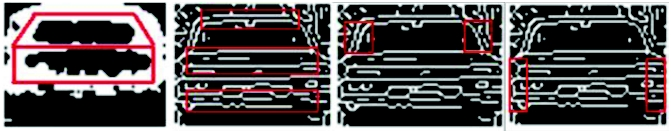
\includegraphics[width=3.15in]{images/hog.jpg}
  \caption{Sub regions with strong orientation of front/rear view car, from left to
right: edge image, horizontal, diagonal and vertical.}
  \label{fig:hog}
\end{figure}
The orientation is ranged in $[0, 2\pi]$, divided into $16$ bins: $h[0]...
h[15]$. For each sub region, we calculate histogram of orientation in
that region by quantizing the orientation $\theta(x, y)$ for all pixels falling
to $h[i]$ bins, $i=\overline{0,15}$, weighted by its magnitude $m(x, y)$.
Condition for input image satisfies orientaiton is that
\begin{equation}
    \begin{array}{rcl}
   H(S) = \left\{ 
   \begin{array}{rcl}
   1 & \mbox{~~} & \frac{h[0] + h[15] + h[7] + h[8]}{\sum_{i=0}^{15}h[i]} > \sigma_1\\
   0 & \mbox{~~} & else
   \end{array}\right. \\
   V(S) = \left\{ 
   \begin{array}{rcl}
   1 & \mbox{~~} & \frac{h[3] + h[4] + h[11] + h[12]}{\sum_{i=0}^{15}h[i]} > \sigma_2\\
   0 & \mbox{~~} & else
   \end{array}\right. \\
   D(S) = \left\{ 
   \begin{array}{rcl}
   1 & \mbox{~~} & \frac{h[1] + h[2] + h[9] + h[10]}{\sum_{i=0}^{15}h[i]} > \sigma_3\\
   0 & \mbox{~~} & else
   \end{array}\right. 
    \end{array}
\end{equation}
where $\sigma_1$, $\sigma_2$, and $\sigma_3$ are specific thresholds. If all sub-regions satisfy
conditions of the strong orientation respectively then input image
satisfies orientation.

Our proposed scheme is evaluated on eight object-categories,
including front/rear view car, side view car, bicycle, train, aeroplane,
motorbike, sheep and horse. We use CALTECH256, UIUC and
PASCAL-VOC 2010 database. Beside, in order to evaluate the result
more exactly, an additional about 1500 negative examples are
collected randomly and added to the database. Thus with each
object-category, the whole database contains about more than 1500
negative images and 1500 positive images (including 1000 images
for training, and 500 images for testing).
%The database contains natural images that are taken from several sources and include occlusion and cluttered backgrounds. 
%With side view car, images used for training have the same size 40x100 as in original database. Otherwhile, all images in the training set of front/rear view car, we resize manually into $60\times80$ to eliminate the influence from background. Similar to other object, 
In the training stage, we choose the basic size for every object. But in the detecting
phase, with an input image, we preprocess it by resizing it into four
times as size of the training image. After detecting at this scale, we reduce it size and continue detect
until the size equals to the training image. By doing that, it is able to
detect all objects in the input image even if the size of object in it is
smaller or larger than the basic size, although it consumes more time
than detecting at a specific scale.
%\small
%\begin{tabular}{p{3.5cm}p{8cm}p{5cm}}
\begin{table}[htbp]
\small
\begin{tabular}{c}%p{3.5cm}p{8cm}p{5cm}}
   \begin{tabular}{|c|c|c|c|c|c|} \hline
	Set & No. image & Correct & In-correct & False rate & Accuracy \\ \hline
	Calt 101 & 504 & 481 & 23 & 4.57\% & 95.43\% \\ \hline
	Calt 256 & 526 & 475 & 41 & 8.95\% & 92.05\% \\ \hline
	Non- car & 665 & 624 & 41 & 6.17\% & 93.83\% \\ \hline
	\end{tabular} \\ %\hline
	Detection result of front/rear view car \\ %\hline
	\begin{tabular}{|c|c|c|c|c|c|} \hline	
	Set & No. image & Correct & In-correct & False rate & Accuracy \\ \hline
	UIUC1 & 300 & 275 & 25 & 8.33\% & 91.67\% \\ \hline
	UIUC2 & 278 & 264 & 14 & 5.04\% & 94.96\%  \\ \hline
	Non- car & 665 & 638 & 27 & 4.06\% & 95.94\% \\ \hline
	\end{tabular} \\ %\hline 
	Detection result of side view car \\ %\hline
\end{tabular}
\caption{The result of our car detecting system.}
\label{table:car_detecting_result}
\end{table}
The final result of our system for car detection is shown in table~\ref{table:car_detecting_result}. The performance of Zhenfeng Zhu~\cite{zhu2004car} (with the same database: Caltech and UIUC) reaches the highest accurate rate at $90.5\%$, while
the lowest accurate of our sytem is about $91.67\%$. This shows that our schema get a better perfomance. Some examples of correct/incorrect detection are shown in Fig~\ref{fig:bicyle_plane_example}. 
%The last image in Fig. 9 presents the positive false of bicycle, while in Fig. 10 it is the negative false of areo plane.
\begin{figure}[ht]
  \centering
  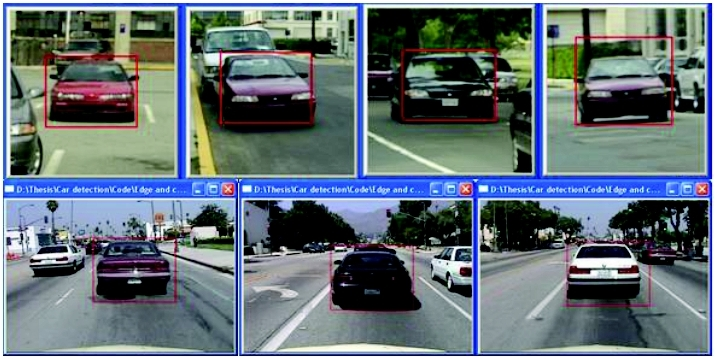
\includegraphics[width=3.15in]{images/car_example.jpg}
  \caption{The true positive detection with front/rear view car.}
  \label{fig:car_example}
\end{figure}
\begin{figure}[ht]
  \centering
  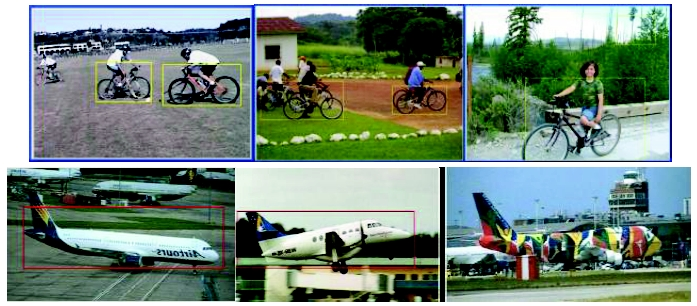
\includegraphics[width=3.15in]{images/bicycle_plane_example.jpg}
  \caption{Bicyle (top) and areoplane (bottom) detection result.}
  \label{fig:bicyle_plane_example}
\end{figure}
We use two ways to check if edge/corner pixel is at right position or
not. One is that if no-pixel in map and no-pixel in mage, then result
is not right $(0\times 0=0)$; other is that no-pixel in map, no-pixel in image,
the result is between right and not-right $(0\times 0=0.5)$. Because if there
is no-pixel in map and no-pixel in testing image, it mean that there
is no edge/corner at that position. That is also a good hint for
regconize object. The final average precision (AP), average recall
(AR) of these two methods is shown in table~\ref{table:compare_0_5}.
%\begin{table}[htbp]
%\small
%\begin{tabular}{|c|c|c|}%p{3.5cm}p{8cm}p{5cm}} 
%    \hline
%	Object & 
%	  \begin{tabular}{c} \hline
%	  $0\times 0 = 0$ \\ \hline
%		  \begin{tabular}{c|c} \hline
%		   AP & AR \\ \hline
%		  \end{tabular}	  
%	  \end{tabular} &
%	  \begin{tabular}{c} 
%	  $0\times 0 = 0.5$ \\ \hline
%		  \begin{tabular}{c|c} \hline
%		   AP & AR \\ \hline
%		  \end{tabular} 
 %	  \end{tabular}  \\ \hline
%\end{tabular}
%\caption{The result of our car detecting system.}
%\label{table:car_detecting_result}
%\end{table}
\begin{table}[htbp]
\small
\begin{tabular}{|c||c|c||c|c|}%p{3.5cm}p{8cm}p{5cm}} 
    \hline 
     Object &  AP (0x0=0) & AR(0x0=0) & AP (0x0=0.5)  & AR(0x0=0.5)  \\ \hline 
     F/r car & 97.40\% & 89.71\% & & \\ \hline
     Side car & 95.83\% & 92.38\% & & \\ \hline
	 Bike & 83.76\% & 72.64\% & 83.82\% & 78.46\% \\ \hline
	Train & 84.05\% & 74.10\% & 81.57\% & 76.43\% \\ \hline
	Aero plane & 85.59\% & 87.56\% & 81.15\% & 86.54\% \\ \hline
	Motorbike & 95.63\% & 85.35\% & 95.35\% & 84.47\% \\ \hline
	Horse & 88.64\% & 68.78\% & 88.37\% & 70.72\% \\ \hline
	Sheep & 74.84\% & 65.96\% & 86.13\% & 71.93\% \\ \hline 
\end{tabular}
\captionof{table}{Comparision between $0\times 0=0$ and $0\times 0=0.5$}
\label{table:compare_0_5}
\end{table}
If there are many edge/corner inside object (such as aero plane,
motorbike), then the $0\times 0=0$ method is better. Otherwhile, if object
doesn t include a lot of edge/corner (bike, horse, sheep or animal is
example), the $0\times 0=0.5$ method will get the higher perfomance. In the
case there are a few of edge/corner on the surface of object (ex.
train), both $0\times 0=0$ and $0\times 0=0.5$ do the same function, and the result
is not different so much.
\subsection{Automatic feature selection for object detecting}
In our experiments below we evaluate the performance of
automatically choosing semantic attribute features on the large data
set used in the 2009, 2010 PASCAL VOC challenge. We believe this
is the first time that the performance of automatically choosing
features has been tested on a standard object classification
benchmark.
In previous section, our system can detect eight categories with
satisfactory result. We combine many features for every object. But
which one category, we must decide which feature is used for
detecting by ourselves. For example, to detect a bike, circle feature is
a good choice, because most of bikes have two wheels with circle
shape. With horse or sheep ojbect, color is a good hint 
due to the fact that the color space of horse or sheep does not change dramatically. With SURF and HoG
feature, because these features are not visual, it is difficult to determine they are suitable for one object or not. In this part, we will evaluate our proposed method in section $4$ for automatically choosing features. We first test with seven features:
edge, corner, HoG, cirle, line, SURF and color. Bias $\omega_p$ and $\omega_n$ are set to $0.6$ and $0.4$ respectively.
\begin{table}[htbp]
\small
\begin{tabular}{|c|c|c|c|c|c|c|c|}%p{3.5cm}p{8cm}p{5cm}} 
    \hline
    Object & Edge & Corner & Line & Circle & HoG & SURF & Color \\ \hline
	F/r car & 1 & 1 & 0 & 0 & 1 & 1 & 0  \\ \hline
	Side car & 1 & 1 & 0 & 1 & 1 &  1 & 0  \\ \hline
	Bike & 1 & 1 & 1 & 1 & 0 & 0 & 0  \\ \hline
	Train & 1 & 1 & 0 & 0 & 1 & 1 & 0  \\ \hline
	Aero plane & 1 & 1  & 1 & 0 & 0 & 1 & 0  \\ \hline
	Motorbike & 1  & 1 & 0 & 0 & 0 & 1 & 1  \\ \hline
	Horse & 1 &  1 & 1 & 0 & 0 & 1 & 1  \\ \hline
	Sheep & 1 & 1 & 0 & 0 & 0 & 1 & 1  \\ \hline
	Tower & 1 & 1 & 1 & 0 & 1 & 0 & 0  \\ \hline
	Flower & 1 & 1 & 0 & 0 & 1 & 1 & 0  \\ \hline
\end{tabular}
\captionof{table}{Object with automatically chosen features}
\label{table:auto_feature_select}
\end{table}
Result of automatically choosing features is in table~\ref{table:auto_feature_select}, where
zero$(0)$ means that feature is not good for object, and one$(1)$
represents we should use this feature to detect object. The image
database for testing automatically choosing feature is same with the
image database for object detecting in section 5.1. The outcome of
this algorithm is predictable, it is almost fit with what we have done
by hand. Only one thing is not as we though is that color feature is
useful for motorbike object (value $1$ at the cell of column Color and
row Motorbike). After checking the motorbike database, we
recognize that most of motorbike-images from CALTECH 256 have
white background and their colors only vary in green, brown, red.
That is the reason why with this database, color is helpful for
detecting motorbike object.
\begin{figure}[ht]
  \centering
  \includegraphics[width=3.35in,height=1.2in]{images/output.pdf}
  \caption{Satisfied, positive and negative score of horse object(left) and side view car(right) .}
  \label{fig:auto_selection}
\end{figure}
In the fig~\ref{fig:auto_selection}, detail of automatically choosing feature for
horse object and side view car object is described. 
%From set of features, we choose one feature with the highest satisfied score (calculated as in section 4). We combine every feature with the first chosen feature, and then we recalculate the satisfied score. We will pick the feature which makes the satisfied score maximum. This feature then is moved to chosen feature set. Next running time, both two chosen features are integrated with new one to compute new satisfied score. By doing this way, 
%The satisfied score increases slowly until it rises to a superior value, which is the maximum value. After that, if more features are combined, the result will be worse. If the score is lower than previous continuously in three permutations, our algorithm would be terminated, and reverse to the peak of score. 
At the beginning, with only one feature, generally the positive score $ pos(f_i,F_c) = |sat(F_c \cup \{f_i\}|T_{pos})| * 1/|T_{pos}|$  is very large because the most of images in $T_{pos}$ satisfy
this feature. Other while, the negative score $neg(f_i,F_c) = (|T_{neg}| - |sat(F_c \cup \{f_i\}|T_{neg})| * 1/|T_{neg}|$ is small. When the more features are
added to chosen feature set, the smaller positive score is, and the
larger negative score becomes. Totally, the satisfied score $g(f_i,F_c) = \omega_p * pos(f_i,F_c) + \omega_n * neg(f_i,F_c)$ (with $\omega_p = 0.6$ and $\omega_n = 0.4$), increases
slowly until it rises to a superior value, represented by the red line. After
this peak, if more features are integrated into $F_C$, the satisfied score
gets lower value.
If the score is lower than the previous one continuously in $k$ permutations, our algorithm would be terminated, and reverse to the peak of score (in our
evaluation, k = 3). Only features before the score gains the peak (on the left side of the red line) will be chosen as strong representative features for that object. For example, with horse object these are chosen-features: CL(color), C(corner), L(line), E(edge) and S(SURF). Other while, with side-view car, H(HoG) is the best feature following by E(edge), CR(circle), E(edge) and C (corner).











\section{Exposition}

aliquip ex ea commodo consequat. Duis aute irure dolor in
reprehenderit in voluptate velit esse cillum dolore eu fugiat nulla
pariatur. Excepteur sint occaecat cupidatat non proident, sunt in
culpa qui officia deserunt mollit anim id est laborum.

\begin{equation}
 \sum_{j=1}^{z} j = \frac{z(z+1)}{2}
\end{equation}

\begin{eqnarray}
x & \ll & y_{1} + \cdots + y_{n} \\
  & \leq & z
\end{eqnarray}

Lorem ipsum dolor sit amet, consectetur adipisicing elit, sed do
culpa qui officia deserunt mollit anim id est laborum.

\section{Exposition}


culpa qui officia deserunt mollit anim id est laborum.
\begin{figure}[ht]
  \centering
  \includegraphics[width=1.5in]{images/samplefigure}
  \caption{Sample illustration.}
\end{figure}

\section{Conclusion}

Lorem ipsum dolor sit amet, consectetur adipisicing elit, sed do
eiusmod tempor incididunt ut labore et dolore magna aliqua. Ut enim ad, sunt in
culpa qui officia deserunt mollit anim id est laborum.

\section*{Acknowledgements}

To Robert, for all the bagels.

\bibliographystyle{acmsiggraph}
\bibliography{ntbaovn-acmsiggrahp2011}
\end{document}
